\documentclass{article}
\setcounter{tocdepth}{4} %Required to insert paragraph in TOC
\setcounter{secnumdepth}{4} %Required to insert paragraph in TOC

\usepackage{graphicx} % Required for inserting images
\graphicspath{ {./img/} }

\usepackage{blindtext}
\usepackage{titlesec}
\usepackage[dvipsnames]{xcolor}
\usepackage{geometry}
\geometry{
	a4paper,
	total={170mm,257mm},
	left=25mm,
	top=20mm,
}

\usepackage{adjustbox}
\usepackage{amsmath}
\usepackage{amssymb}
\usepackage{cancel}
\usepackage{caption}
\usepackage{subcaption}
\usepackage{titlesec}
\usepackage{float}
\usepackage{enumitem}
\usepackage{hyperref}
\usepackage{makecell}
\usepackage{chronology}
\usepackage{cleveref}

\setcounter{secnumdepth}{4}

\newcommand{\foo}{\hspace{-2.3pt}$\bullet$ \hspace{5pt}}

\titleformat{\paragraph}
{\normalfont\normalsize\bfseries}{\theparagraph}{1em}{}
\titlespacing*{\paragraph}
{0pt}{3.25ex plus 1ex minus .2ex}{1.5ex plus .2ex}

\title{Appunti Basi di Dati}
\author{Mattia Robuschi Caprara}
\date{}

\definecolor{CoverGreen}{RGB}{229,190,001}

\begin{document}
	
	\begin{titlepage}
		
		\pagecolor{CoverGreen}
		
		\vspace{25 mm}
		\begin{center}
			\large
			{\color{black}\textbf{Mattia Robuschi Caprara}} 
		\end{center}
		
		\begin{center}
			\huge
			{\color{black}\textbf{Basi di Dati}}
		\end{center}
		
		\vspace{45 mm}
		
		\begin{figure}[h]
			\centering
			\adjustbox{cfbox=white 5pt 0cm}{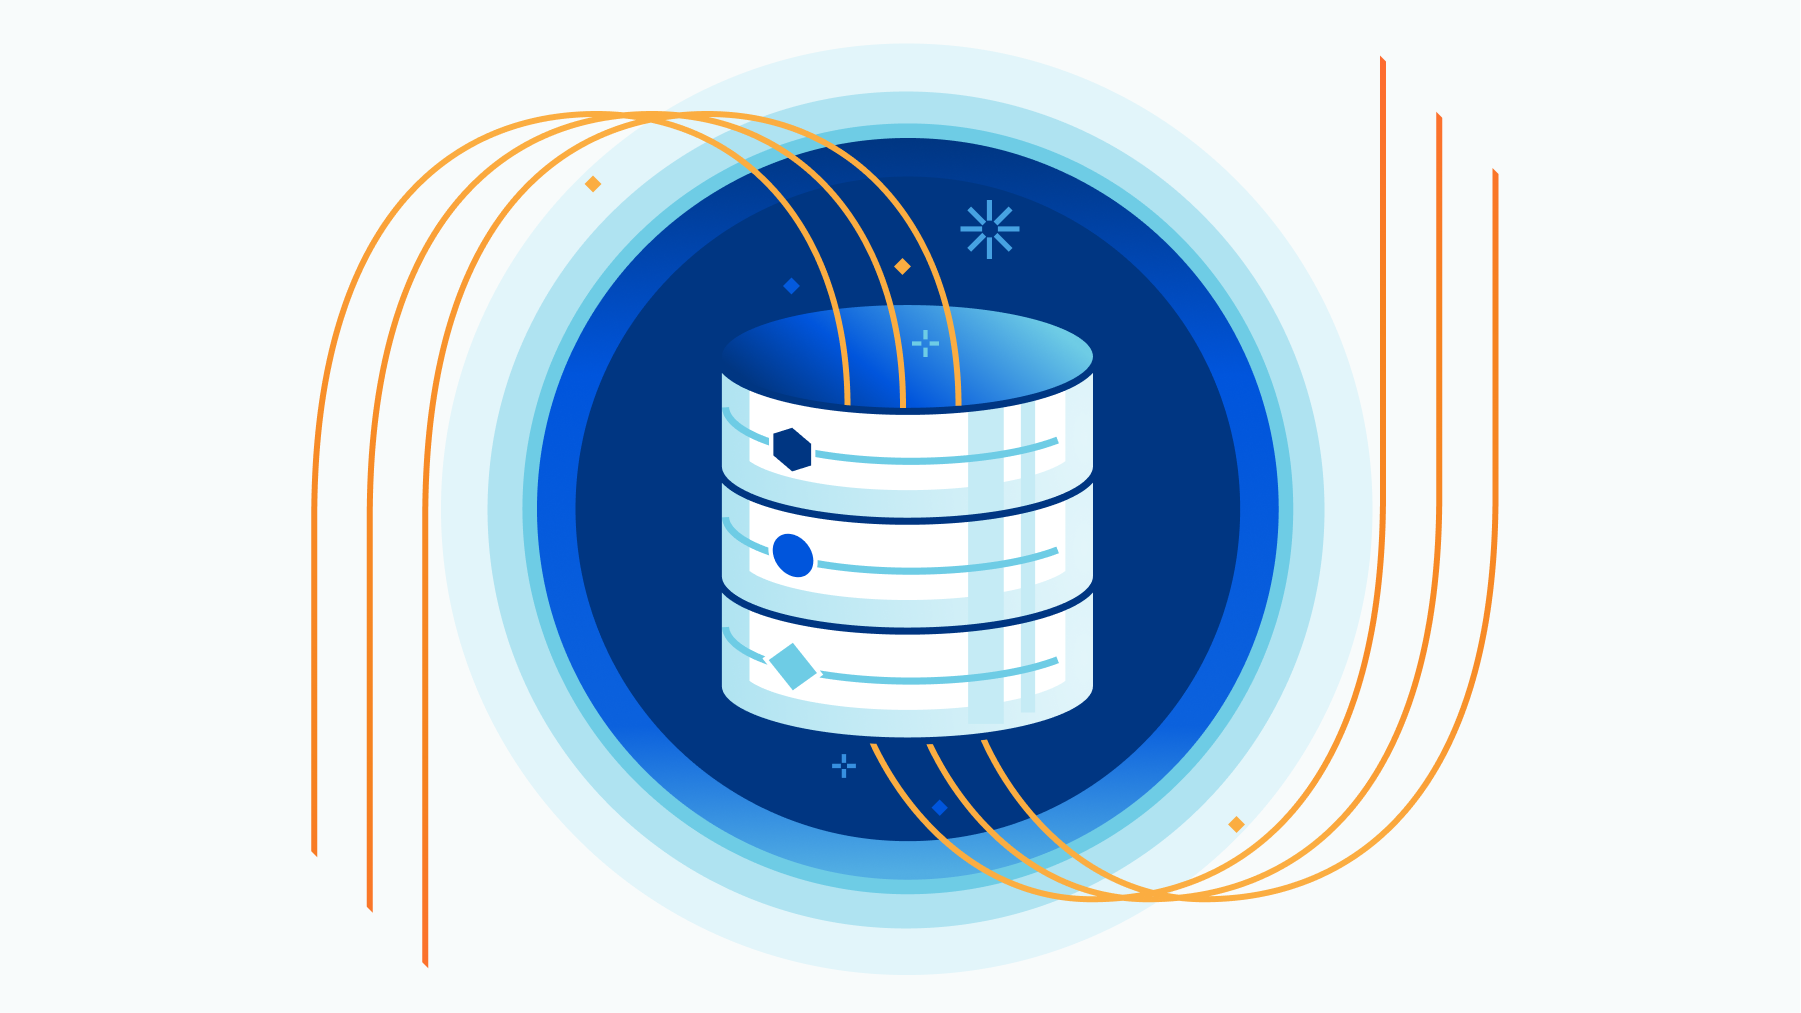
\includegraphics[scale=0.18]{0.cover.png}}
			%\caption{Caption}
			\label{fig:cover}
		\end{figure}
		
		\thispagestyle{empty} 
	\end{titlepage}
	
	\newpage
	\pagecolor{white}
	\section*{Prefazione}
	\textbf{!!ATTENZIONE!!}\\
	Questo documento è un semplice OCR delle slide del prof.\\ \\
	Scopo (pratico) del corso\\
	Nel corso vedremo (parzialmente in parallelo):\\
	\begin{enumerate}
		\item 	Come progettare una base di dati sulla base delle specifiche che vengono fornite. \\
		(progettazione concettuale progettazione logica normalizzazione)
		\item Come gestire e interrogare la base di dati, una volta che è stata realizzata e "popolata".\\
		(modello relazionale, linguaggio SQL)
		\item 	Come gestire gli accessi concorrenti alla base di dati da parte di più utenti, ma in modo sicuro (nel senso della correttezza del risultato) (transazioni)
		\item Esempi di DB non relazionali (NoSQL)
	\end{enumerate}
	\tableofcontents
	\newpage
	
	\section{Basi di Dati}
	\textbf{Informazione}: notizia, dato o elemento che consente di avere conoscenza più o meno esatta di fatti, situazioni, modi di essere\\
	\textbf{Dato}: ciò che è immediatamente presente alla conoscenza, prima di ogni elaborazione; (in informatica) elemento di informazione costituito da simboli che devono essere elaborati (dal Vocabolario della Lingua Italiana, Istituto dell’Enciclopedia Italiana)\\
	\textbf{Base di Dati}: collezione di dati, utilizzati per rappresentare le informazioni di interesse per un sistema informativo
	\section{Architettura Client-Server}
	\begin{figure}[h]
		\centering
		\adjustbox{cfbox=white 5pt 0cm}{\includegraphics[scale=0.3]{example-image-golden}}
		\caption{Caption}
		\label{fig:im-1}
	\end{figure}
	Architettura client-server (applicazione lato server)\\
	DBMS (MySQL/MariaDB), Server Web (APACHE) e interprete PHP sono integrati nel pacchetto XAMPP, scaricabile da questo \href{https://www.apachefriends.org/it/download.html}{link}\\
	L'applicazione risiede sulla macchina dell'utente e può essere scritta in qualsiasi linguaggio dotato di una API per connettersi, come nel caso di un browser, a un server web (protocollo HTTP) e/o a un server SQL.
	\section{DBMS}
	Un Database Management System (DBMS) è un sistema software che si interpone fra le applicazioni e la memoria di massa in cui si trovano collezioni di dati.\\
	La finalità di un DBMS è l’estensione delle funzionalità del file system, in modo da offrire:
	\begin{itemize}
		\item Nuove modalità di accesso ai dati
		\item Condivisione dei dati
		\item Gestione più sofisticata dei file
	\end{itemize}
	Le basi di dati gestite dai DBMS sono collezioni di dati:
	\begin{itemize}
		\item \textbf{Grandi} possono avere notevoli dimensioni (fino a centinaia di Terabyte) e devono quindi necessariamente risiedere nella memoria secondaria
		\item \textbf{Condivise} applicazioni ed utenti diversi devono potere accedere ai dati
		\item \textbf{Persistenti} Il tempo di vita dei dati va oltre la durata dell’esecuzione delle singole applicazioni
	\end{itemize}
	Un DBMS deve garantire:
	\begin{itemize}
		\item Affidabilità 
		\item Privatezza dei dati 
		\item Efficienza 
		\item Efficacia
	\end{itemize}
	\subsection{Affidabilità}
	Un DBMS deve garantire di poter mantenere intatto il suo contenuto, anche in caso di malfunzionamento.\\
	L’integrità dei dati è affidata a procedure di backup (salvataggio) e recovery (recupero) dei dati, o alla loro duplicazione nei casi più critici.
	\subsection{Privatezza dei dati}
	Ogni utente, abilitato a utilizzare la base di dati attraverso una procedura di riconoscimento, può accedere ad insiemi limitati di dati e compiere solo certe operazioni su di essi.
	\subsection{Efficienza}
	Un DBMS deve operare e fornire risposte agli utenti in tempi accettabili, utilizzando una quantità il più possibile limitata di risorse.\\
	L’efficienza dipende essenzialmente dalle tecniche utilizzate per l’implementazione del DBMS e dalla buona progettazione della base di dati.\\
	Si misura (come in tutti i sistemi informatici) in termini di tempo di esecuzione (tempo di risposta) e spazio di memoria (principale e secondaria) occupato.
	\subsection{Efficacia}
	Capacità di un DBMS di rendere produttive le attività degli utenti, cioè di consentire la realizzazione di basi di dati che risolvano in modo efficace i problemi degli utenti.\\
	Concetto generico, qualitativo e non legato a specifiche funzionalità del DBMS.\\
	Non esistono criteri oggettivi per valutarla.
	\subsection{Indipendenza dei dati}
	Il nuovo strato che il DBMS viene a creare fra memoria di massa e applicazioni consente di conservare e gestire i dati in modo indipendente dalle applicazioni stesse.\\
	Normalmente le applicazioni accedono a dati locali gestendoli attraverso file che appartengono alle applicazioni stesse.\\
	In presenza di un DBMS, i dati non appartengono ad una specifica applicazione, ma le diverse applicazioni vi accedono attraverso di esso.
	\section{Modelli dei Dati}
	La progettazione di una base di dati si svolge attraverso una serie di fasi successive, identificabili come:
	\begin{itemize}
		\item Raccolta delle specifiche (identificazione dei concetti)
		\item Progettazione concettuale
		\item Progettazione logica
		\item Progettazione fisica (non compresa nel corso)
	\end{itemize}
	Ogni fase fa riferimento ad un modello dei dati che corrisponde ad un meccanismo di strutturazione dei dati attuato a soddisfare le finalità della corrispondente fase della progettazione.\\
	Un modello di dati è costituito dai concetti sulla base dei quali i dati sono strutturati e codificati.\\
	Ogni modello di dati fornisce meccanismi di strutturazione dati, analoghi ai costruttori di tipo dei linguaggi di programmazione.\\
	I modelli concettuali descrivono la realtà mediante concetti astratti, ma soggetti a precise regole.\\
	Non sono finalizzati alla rappresentazione dei dati nel calcolatore, ma a descrivere (e caratterizzare per ruolo) i concetti del mondo reale di cui i dati sono istanze.\\
	Si usano nella fase di progettazione concettuale.\\
	Nel corso useremo il modello Entità/Relazione.
	\begin{figure}[h]
		\centering
		\adjustbox{cfbox=white 5pt 0cm}{\includegraphics[scale=0.3]{example-image-golden}}
		\caption{Modello (concettuale) entità-relazione}
		\label{fig:im-2}
	\end{figure}\\ 
	Si esprimono i concetti che devono essere rappresentati dai dati come concetti indipendenti (entità) e relazioni logiche che li collegano (relazioni) e che esistono solo in presenza delle entità.\\
	I DBMS si differenziano in base al modello logico che utilizzano.\\
	Quindi i modelli logici, seppure astratti come i modelli concettuali, non hanno solo finalità descrittive e di documentazione, ma riflettono la struttura con cui i dati sono organizzati all’interno del calcolatore.
	\subsection{Il problema fondamentale}
	Dato un frammento della realtà che può essere identificato e isolato rispetto al "resto del mondo":
	\begin{itemize}
		\item Descriverlo nel modo più completo possibile, identificando tutti gli elementi (concetti) che lo compongono (e che permettono di distinguerlo da tutto il resto)
		\item Descrivere, a sua volta, ogni elemento nel modo più corretto possibile, identificandone tutte le caratteristiche (attributi) che permettono di caratterizzarlo nel contesto considerato e ignorando quelle superflue rispetto a tale contesto
	\end{itemize}
	Se abbiamo identificato più concetti, questi dovranno risultare logicamente collegati fra loro: ogni concetto deve essere collegato ad almeno un altro concetto, in modo che non vi sia alcun concetto (o insieme di concetti) "isolato" dagli altri.\\
	Se così fosse, infatti, questo costituirebbe un secondo frammento della realtà indipendente da quello considerato e non avrebbe senso descriverli insieme.\\
	Fra i concetti, alcuni (entità) potranno essere descritti in modo indipendente dagli altri attraverso un insieme di attributi che gli sono propri e tipici, senza bisogno di fare riferimento ad altri concetti.\\
	Ad esempio, se il contesto è la gestione di un negozio, posso descrivere un prodotto attraverso il nome, il peso, il prezzo, ecc... e posso descrivere un cliente attraverso i suoi dati anagrafici.\\ \\
	Però non basta, due concetti che posso descrivere in modo indipendente l’uno dall’altro come cliente e prodotto non possono costituire la descrizione completa di un contesto comune.\\
	Per descrivere il contesto del negozio, quindi, cliente e prodotto non possono fare parte della stessa descrizione (schema) senza che esista (almeno) un altro concetto che li colleghi.\\
	D’altra parte, ovviamente, un tale concetto non può, in alcun caso, essere indipendente e non può essere descritto senza fare riferimento ai concetti che collega.\\
	Un concetto che collega altri concetti, e che quindi non può esistere se non esistono i concetti che collega, si chiama relazione o associazione.\\ \\
	Nel caso del negozio, dato il concetto di cliente e di prodotto, una possibile associazione sufficiente a completare lo schema è VENDITA \\ \\
	Ancora non basta, una relazione è un concetto che non è descrivibile soltanto attraverso i riferimenti agli altri concetti (anche più di due) che collega, ma è anch’essa caratterizzata da specifici attributi.\\
	Ad esempio, la descrizione di una vendita dovrà necessariamente contenere l’informazione relativa al cliente cui viene venduto un prodotto e al prodotto che ne è oggetto, ma potrà (e dovrà) anche specificare:
	\begin{itemize}
		\item Data della vendita 
		\item Quantità del prodotto venduto 
		\item Prezzo unitario del prodotto o prezzo totale
		\item Numero della fattura in cui viene riportata (in questo caso sarà necessario definire un’entità Fattura a cui fare riferimento, quindi estendere lo schema)
	\end{itemize}
	\subsection{Modelli logici dei dati}
	\begin{itemize}
		\item \textbf{Relazionale}: Il più diffuso, basato su un modello tabellare dei dati
		\item \textbf{Gerarchico}: Utilizzato nei primi DBMS (anni 60), tuttora utilizzato, basato su strutture ad albero
		\item \textbf{Reticolare}: Estensione del modello gerarchico, basato su grafi
		\item \textbf{A oggetti}: Estensione del modello relazionale basato sui paradigmi OOP.
		\item \textbf{XML (semistrutturato)}: Deriva dal modello gerarchico, ma è più flessibile
	\end{itemize}
	\subsection{Modello relazionale}
	E’ un modello logico: definisce tipi attraverso il costruttore relazione, che organizza i dati secondo record a struttura fissa, rappresentabili attraverso tabelle.\\
	Es. (relazioni INSEGNAMENTO e MANIFESTO)\\
	\begin{table}[ht]
		\begin{minipage}{.5\linewidth}
			\centering
			\begin{tabular}{ |c|c|  }
				\hline
				\textbf{Corso} & \textbf{Titolare} \\
				\hline
				Basi di Dati e Web & Cagnoni \\
				Fondamenti di Informatica & Tomaiuolo\\
				Ingegneria Del Software & Poggi \\
				\hline
			\end{tabular}
			%\caption{Caption}
		\end{minipage}
		\hfill
		\begin{minipage}{.5\linewidth}
			\centering
			\begin{tabular}{ |c|c|c|  }
				\hline
				\textbf{CdL} & \textbf{Materia} & \textbf{Anno}\\
				\hline
				IET-I & Basi di Dati e Web & 3 \\
				IET & Fondamenti di Informatica& 1\\
				IET-I & Ingegneria del Software & 3\\
				\hline
			\end{tabular}
			%\caption{Caption}
		\end{minipage}
	\end{table}
	\subsection{Schema}
	In ogni base di dati si possono distinguere:
	\begin{itemize}
		\item \textbf{Lo schema}, sostanzialmente invariante nel tempo. Ne descrive la struttura (si parla di aspetto intensionale).\\
		Nell’esempio, le tabelle e le "intestazioni" delle tabelle\\
		Analogo della definizione di una classe in un linguaggio a oggetti
		\item \textbf{Le istanze}, cioè i valori attuali, che possono cambiare anche molto rapidamente (si parla di aspetto estensionale).\\
		Nell’esempio, i singoli dati contenuti in ciascuna tabella\\
		A livello concettuale, analogo di un oggetto, come istanza di una classe, in un linguaggio a oggetti
	\end{itemize}
	Lo schema di una base di dati è la parte dichiarativa ed invariante della base di dati e ne definisce la struttura.\\
	Nel modello relazionale lo schema di una relazione è paragonabile alla definizione del prototipo di una funzione in C:\\ \\
	INSEGNAMENTO (Corso, Titolare)\\ \\
	è lo schema della relazione INSEGNAMENTO definita su due attributi (campi del record identificati da una etichetta che ne descrive il significato).\\
	Le n-ple di attributi appartenenti alla relazione, a ciascuno dei quali deve essere assegnato un valore, sono dette istanze della relazione.\\ \\
	(Basi di dati, Cagnoni) è una istanza di INSEGNAMENTO\\ \\ \\
	Gli schemi possono operare a diversi livelli di astrazione.\\
	Dalle specifiche è possibile derivare lo \textbf{Schema concettuale} che descrive i concetti che devono essere rappresentati, i dettagli che servono per descriverli e le relazioni logiche che li collegano.\\ \\
	Dallo schema concettuale si deriva lo \textbf{Schema logico} che descrive la struttura dell’intera base di dati mediante il modello logico adottato dal DBMS (reticolare, gerarchico, relazionale).\\ \\
	Che viene poi realizzato attraverso lo \textbf{Schema interno (o schema fisico)} che implementa lo schema logico mediante strutture fisiche di memorizzazione\\ \\
	Nei confronti dell’utente è possibile definire anche uno \textbf{Schema esterno} che descrive la struttura di una porzione della base di dati attraverso il modello logico, dal punto di vista di una classe di utenti.\\
	Generalmente realizzato mediante viste, relazioni derivate da quelle che costituiscono lo schema logico.\\ \\
	Es. (i soli corsi del curriculum Ingegneria Informatica):\\
	\begin{tabular}{ |c|c|c|  }
		\hline
		\textbf{CdL} & \textbf{Materia} & \textbf{Anno}\\
		\hline
		IET-I & Basi di Dati e Web & 3 \\
		IET-I & Ingegneria del Software & 3\\
		\hline
	\end{tabular}
	\begin{figure}[h]
		\centering
		\adjustbox{cfbox=white 5pt 0cm}{\includegraphics[scale=0.3]{example-image-golden}}
		\caption{Architettura standard (ANSI/SPARC) a tre livelli per DBMS}
		\label{fig:im-3}
	\end{figure}
	\newpage
	\section{Progettazione di una base di dati}
	I diversi tipi di schema riflettono le diverse fasi della progettazione: date le specifiche del problema da risolvere
	\begin{itemize}
		\item \textbf{Progettazione concettuale} (dalle specifiche allo schema concettuale) \\
		Definisce quali concetti rappresentare, per quanto riguarda sia la loro descrizione che le relazioni logiche che esistono fra di essi.
		\item \textbf{Progettazione logica} (dallo schema concettuale allo schema logico) \\
		Definisce come rappresentare i concetti introdotti a livello concettuale in forma di strutture dati.
		\item \textbf{Progettazione fisica} (dallo schema logico allo schema fisico) \\
		Definisce come allocare e gestire fisicamente i dati all’interno del calcolatore.
	\end{itemize}
	

\end{document}